\subsection{Test de tiempo en función de la granularidad de la discretización}
En este test se corrió el algoritmo de Gauss con diferentes grupos de instancias con diferente
granularidad. Empezando desde 50 hasta 104 radios y ángulos, de igual cantidad. Se lo comparó con
una función lineal

\begin{figure}[H]{}
\centering
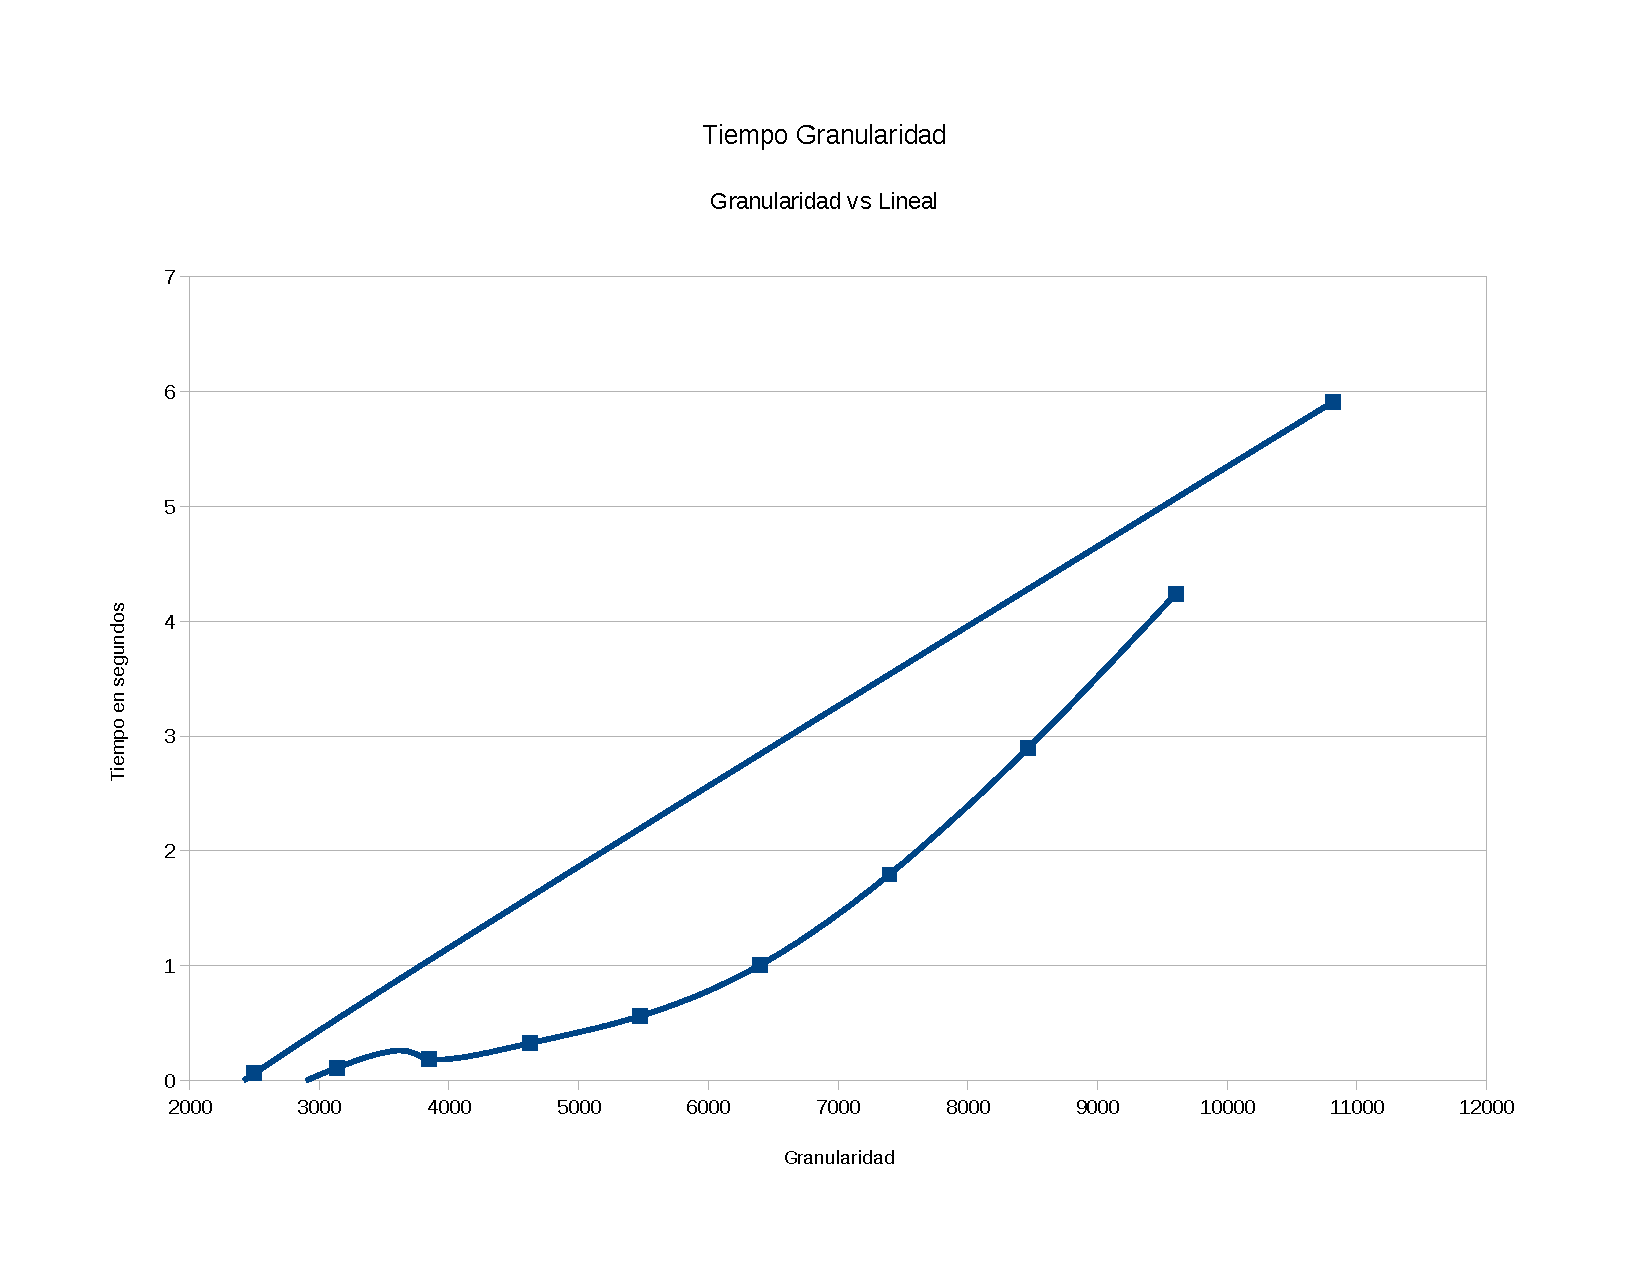
\includegraphics[scale=0.5]{graphs/granuVstiempo.pdf}
\caption{Comparación del tiempo de ejecución de diferentes granularidades con una función lineal.}
\label{gaussVsLU1}
\end{figure}

